% exercise sheet with header on every page for math or close subjects
\documentclass[12pt]{article}
\usepackage{german} 
\usepackage[utf8]{inputenc} 
\usepackage{latexsym} 
\usepackage{multicol}
\usepackage{fancyhdr}
\usepackage{amsfonts} 
\usepackage{amsmath}
\usepackage{amssymb}
\usepackage{enumerate}
\usepackage{MnSymbol}
\usepackage[colorlinks=true,urlcolor=blue]{hyperref}
\usepackage{listings}
\usepackage{graphicx}

% Shortcuts for bb, frak and cal letters
\newcommand{\E}{\mathbb{E}}
\newcommand{\V}{\mathbb{V}}
\renewcommand{\P}{\mathbb{P}}
\newcommand{\N}{\mathbb{N}}
\newcommand{\R}{\mathbb{R}}
\newcommand{\C}{\mathbb{C}}
\newcommand{\Z}{\mathbb{Z}}
\newcommand{\Pfrak}{\mathfrak{P}}
\newcommand{\Pfrac}{\mathfrak{P}}
\newcommand{\Bfrac}{\mathfrak{P}}
\newcommand{\Bfrak}{\mathfrak{B}}
\newcommand{\Fcal}{\mathcal{F}}
\newcommand{\Ycal}{\mathcal{Y}}
\newcommand{\Bcal}{\mathcal{B}}
\newcommand{\Acal}{\mathcal{A}}


% Formatierung
\topmargin -2cm 
\textheight 24cm
\textwidth 16.0 cm 
\oddsidemargin -0.1cm

\setlength{\parindent}{0pt}  % !!!!!!! Hier werden leerzeilen erlaubt ohne dass Latex automatisch einrueckt! !!!!!!! %


%Python code Highlighting
\lstset{language=Python, tabsize=3,
        basicstyle=\ttfamily\small, 
        keywordstyle=\color{keywords},
        commentstyle=\color{comments},
        stringstyle=\color{red},
        showstringspaces=false,
        identifierstyle=\color{green}}

% Code-Highlighting Java
%\lstset{language=Java, breaklines=true, showstringspaces=false}
%\begin{lstlisting}
%    	Hier würde der Java-Code hinkommen und entsprechend die Syntax markiert. Selbst einrücken.
%\end{lstlisting}
%ODER:
% \lstinputlisting[language=Java]{name.py}

\graphicspath{ {images/} }


\begin{document}

% Titel
%\title{\textsc{Hacking}\\ \textsc{Abgabe 0}\\{ \normalsize Gruppe X \hfill Daniel Schäfer (2549458)\\ \hfill Anderer}}
%\maketitle  

% alternativer Titel
\noindent
{\Large \textbf{High-level Computer Vision}} \hfill \textbf{16.05.2016}\\
{\Large \textbf{Exercise 2}} 
\raggedleft \hfill Guillermo Reyes (2556018)\\
\hfill Daniel Schaefer (2549458)\\
\hfill Marc Tonsen(2537359)\\
\hfill Dominik Weber (2548553)\\

\pagenumbering{gobble}
\raggedright


\section*{Code Annotations}




\section*{Question 3: Region Descriptors}

\begin{enumerate}[a)]
	\setcounter{enumi}{3}
	\item 	
	\textbf{Which descriptor performs better and why?}\\
	
	\begin{figure}[h]
		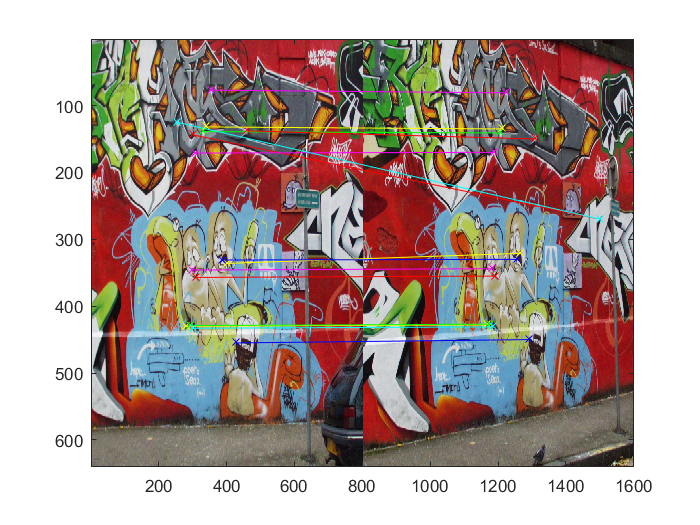
\includegraphics[width=0.5\textwidth]{graf_har_rg}
		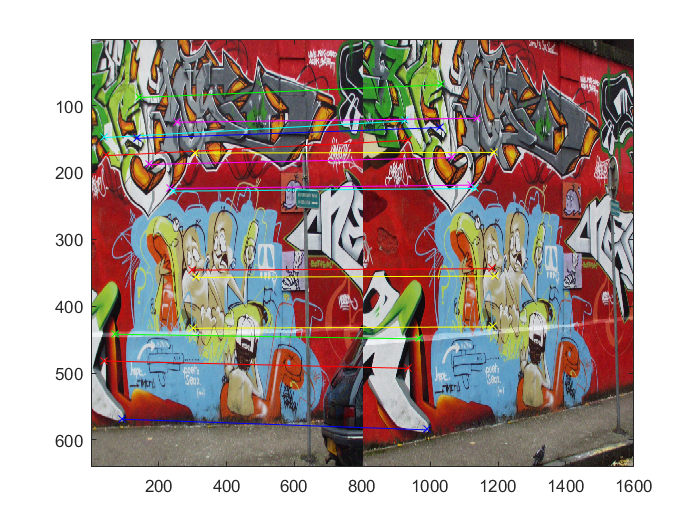
\includegraphics[width=0.5\textwidth]{graf_har_dxdy}
		\caption{\textit{Left}: Harris detector with rg histogram descriptor. \textit{Right}: also Harris, but using the dxdy histogram descriptor }
	\end{figure}

	\begin{figure}[h]			
		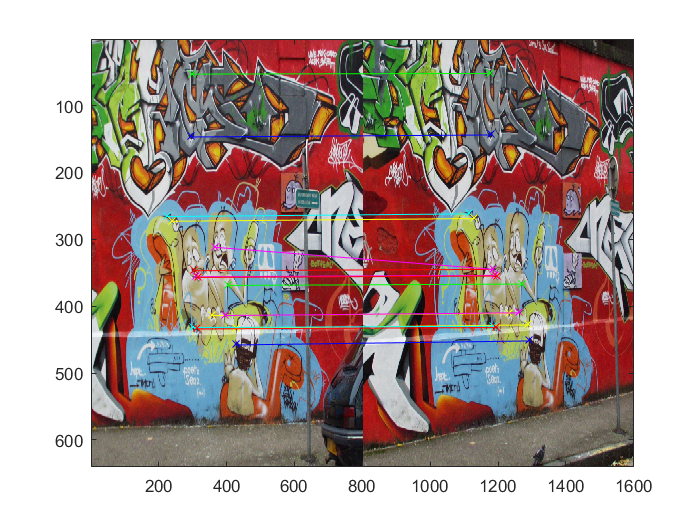
\includegraphics[width=0.5\textwidth]{graf_hes_rg}
		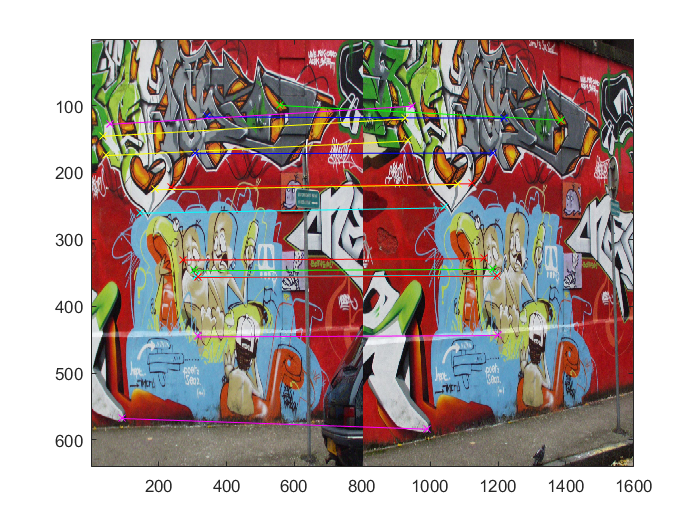
\includegraphics[width=0.5\textwidth]{graf_hes_dxdy}
		\caption{\textit{Left}: Hessian detector with rg histogram descriptor. \textit{Right}: also Hessian, but using the dxdy histogram descriptor }
	\end{figure}
	
	If examined carefully, one can notice from the images in figures 1 and 2 that for both, Harris and Hessian detectors, the dxdy-histogram descriptor seems to outperform the rg-histogram descriptor in this example, based on the amount of mismatched points between the images. This may be due to wo reasons: first, the images present very hard edges which virtually don't change if the angle of the image is changed.This makes it ideal for dxdy as it can more easily distinguish two different sections of the image. Another factor could be that the image itself presents very similar colors in different parts. One such example is on the baby's faces in figure 2 left, where, even though the matched points are close to each other, they do not correspond to the right match. There are of course other more extreme examples where points near some of the letters get matched to points in completely different locations.
	It is important to note, never the less, that this does not mean that using dxdy-histograms is better than using rg-histograms, but is instead domain dependent, and even if dxdy beats rg-histograms in this image, there will be others where it will not be so.
	\item
	
	\begin{figure}[h]
		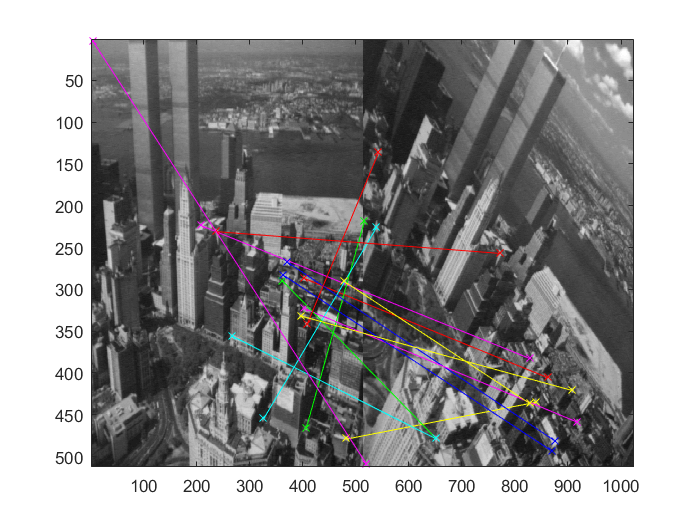
\includegraphics[width=0.5\textwidth]{ny_hes_dxdy}
		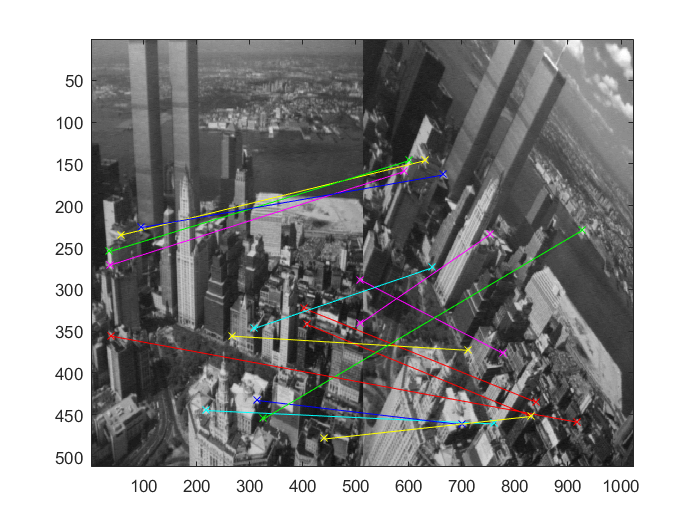
\includegraphics[width=0.5\textwidth]{ny_hes_maglap}
		\caption{\textit{Left}: Hessian detector with dxdy histogram descriptor. \textit{Right}: also Hessian, but using the maglap histogram descriptor }
	\end{figure}
	
	In the case of the New York images, one can see a few more inconsistencies in the case of the dxdy-histogram compared to the graffiti images. This might be because it is an image from a city (3D) no of a graffiti (2D) which means changing the angle of view has a bigger impact on the image and therefore the first derivative, which is what the dxdy-histogram uses. As for the maglap-histogram, one can see less inconsistencies than the dxdy-histogram. It is no surprise that it performs better as it also uses the first derivative, in part, but also the second derivative. So in a way, it is more informed than just the dxdy histogram and can, thus, make better matches. As opposed to the comparison of rg-histograms vs dxdy-histograms one would expect that in general maglap-histograms outperform dxdy-histograms.
	
	\textbf{Summary of observations}\\
    %TODO

\end{enumerate}

\newpage
\section*{Question 4: Panorama Stitching}
\begin{enumerate}[a)]
%	\setcounter{enumi}{2}
	\item 
	\textbf{Homography estimation with RANSAC.}
     \begin{itemize}
     	\item
     	\textbf{What does homography estimation do?}\\
        Homography is the projective transformation between two images of the same planar surface, i.e. it maps the points of one image to the points of another image taken by a camera which was projectively transformed from the first one. To estimate the homography of two images a set of of pairs of points is required, which represent projections of the same world point in each image.\\
        In the case of \verb!get_ransac_hom.m!, it tries to compute the homography as a transformation matrix that transforms one given set of points to another.  In practise a homography can usually not be computed exactly due to noise in the data. Therefore it has to be estimated, for which it is important to 'ignore' outlier data (possible errors in data collection, \dots) to preserve a realistic and precise estimation.

     	\item
     	\textbf{What are the steps of RANSAC algorithm and why it is useful?}\\
        \begin{enumerate}[1)]
            \item 
                We compute a random sample of Data-values
            \item
                We compute the Homography of these randomly selected values
            \item
                We check if this random sample contains more inliers compared to the best random-sample we computed earlier, if that is the case we save our new random sample as the new best random-sample.
            \item
                There is a statistic method which estimates the number of neccessary ransac iterations using the ratio of inliers and outliers. With every iteration we can improve our estimation of neccesary iterations, thats why we update this number every time
            \item 
                Once all iterations are finished, we are going to improve the best sample we found:
                \begin{itemize}
                    \item 
                        Every point inside the threshold around the computed Homography of the best sample found, is used as input set of which the homography is computed again, to enlarge the subset on which our homography is based on. This is done exactly once in our implementation.
                \end{itemize}
            \item
                Now we have succesfully computed the resulting Homography.
        \end{enumerate}

     \end{itemize}
\end{enumerate}


\end{document}
